\documentclass{article}
\usepackage[english]{babel}
\usepackage[utf8]{inputenc}
\usepackage[T1]{fontenc}
\usepackage{amsmath,amssymb,amsfonts}

\usepackage{xspace}
\usepackage{graphicx}

\newcommand{\system}{MADden\xspace}

\title{MADden : In-Database Text Analytics}
\author{Morgan Bauer 9890-4838 \\
  Christan Grant 8143-3970 \\
  Joir-dan Gumbs 6148-9357}
\begin{document}
\maketitle
\begin{enumerate}
\item Names of the group members and UFIDs

  % not sure if it's best to put this into the public with our uf-id on it ~mhb

  Morgan Bauer

  Christan Grant

  Joir-dan Gumbs

\item Title of the project and abstract

  MADden : In-Database Text Analytics

\item Final report should include the following topics:
  \begin{enumerate}

  \item  Introduction (1 page)
    \begin{enumerate}
    \item The problem statement and a summary of the main contributions and results of the project.
    \item What is the responsibility of each member of the group?

      Morgan did consulting work among the various group members, and between groups.
      Official NFL team blogs. NFL stats from cbssports.com.
    \end{enumerate}

  \item Background (1 page)
    \begin{enumerate}
    \item Background information (basic concepts, algorithms, etc.)

      algorithms -- crf (viterbi, forward-backward) evaluation over trained model done in database.

    \item Related work
    \item How is this project different from related work

      integration of analysis queries
    \end{enumerate}

  \item
    \section{System Description (4 pages)}
    \begin{enumerate}
    \item What is the final system architecture?

      {\system} is a four layered system, as can be seen in Figure \ref{fig:arch}.
      The user interface is where both naive and advanced users can construct queries over text, structured data, and models.
      From the user interface,
      queries are then passed to the DBMS,
      where MADLib and {\system} libraries sit on top of the query processor to add statistical and text processing functionality.
      These queries are processed using PostgreSQL/Greenplum's Parallel DB architecture to further optimize on replicated storage.

      \begin{enumerate}
      \item information extraction

        
      \item entity resolution

        This links various forms and representations of the same background object, 
        so that a query for one of them returns the results for all of them.
        This is necessary for two reasons,
        the informality of speaking in documents like blog posts and twitter tweets, 
        which leads to misspellings and slang
        and the more general case of people or companies having many names to refer to them.
        
        Example of informality, slang \& misspelling. tmrw, tomorrow. NY Jest, NY Jets.

        Example of multiple names for a person. Nicknames. IBM, Big Blue. New York City, Big Apple.

      \item sentiment analysis


      \item part of speech tagging

        Using CRF

        Using NLTK.
      \end{enumerate}


      PostgreSQL, with MADlib overtop.

      call to twitter sentiment . This is done as a udf calling python script which uses a JSON API.

      Call to nltk for entity resolution.

      \begin{figure}
        \begin{center}
          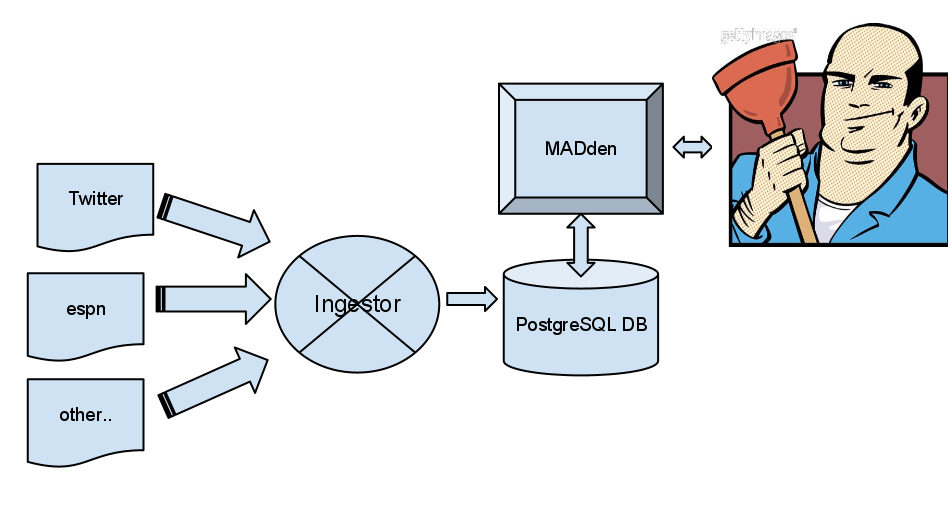
\includegraphics[width=104mm]{architecture-1.png}
          \caption{System Architecture}
          \label{fig:architecture}
        \end{center}
      \end{figure}

      \begin{figure}
        \begin{center}
          \includegraphics[scale=0.4]{arch.png}
          \caption{{\system} architecture}
          \label{fig:arch}
        \end{center}
      \end{figure}

      \begin{figure}
        \begin{center}
          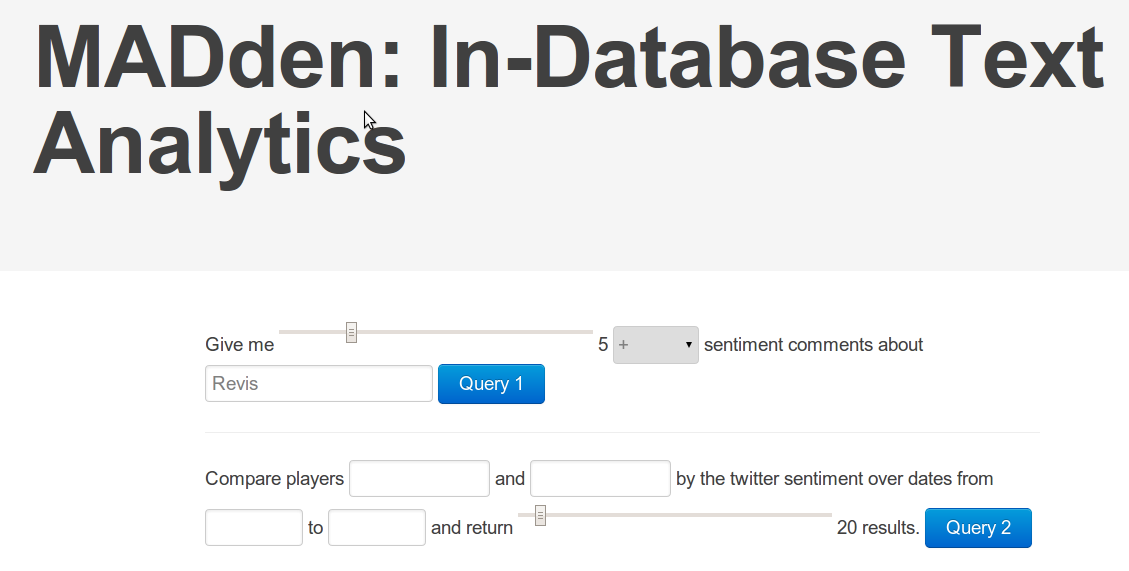
\includegraphics[scale=0.3]{web-ui.png}
          \caption{{\system} Web UI}
          \label{fig:web-ui}
        \end{center}
      \end{figure}

    \item What are the system components and statistical methods developed?

    \item What are the final data products?

      We don't have particular products, so much as abilities to deliver varying products.

      Query results
    \end{enumerate}

  \item Experiments (2 pages)
    \begin{enumerate}
    \item What datasets have been used? What’s the measure of success?

      % my description of document size is vague ~mhb

      Twitter -- unstructured, microblogs, very small document size (140 characters).

      Blogs -- english language, small-medium document size, 10-100 sentences.

      play-by-plays -- semi-structured, repeated patterns with specific meaning.

    \item What are the main experimental results? Effectiveness/performance?
    \end{enumerate}

  \item Conclusion (1 page)
    \begin{enumerate}\item What you have learnt through this project?
      What are the difficulties you have encountered in terms of systems and algorithms in building the system to deliver the data products?
      What kinds of Data Science tools/systems are needed?
    \end{enumerate}
  \end{enumerate}
\end{enumerate}

References

MADlib http://madlib.net/

https://sites.google.com/site/twittersentimenthelp/

\end{document}

%%% Local Variables:
%%% mode: latex
%%% TeX-master: t
%%% End:
